\chapter{Progettazione}
\label{cap:progettazione}

\intro{In questo capitolo si esporranno le caratteristiche tecniche della soluzione prodotta, descrivendo la progettazione e l'architettura adottata di telemetria e test}\\

\section{Osservabilità nei sistemi distribuiti}

L'osservabilità è la proprietà di un sistema software che permette di comprenderne
lo stato interno esaminando esclusivamente i dati prodotti in output. Nel contesto delle
applicazioni web distribuite, questa proprietà è resa possibile dalla produzione
sistematica di tre categorie di segnali:
\begin{itemize}
\item \textbf{Logs}: rappresentano eventi discreti generati dal sistema durante la sua esecuzione. Contengono informazioni dettagliate su operazioni svolte, errori, stati e messaggi diagnostici, risultando fondamentali per attività di debugging e analisi puntuale di anomalie.

\item \textbf{Traces}: descrivono il flusso di esecuzione di una richiesta all’interno del sistema, tracciandone il percorso attraverso i vari componenti e servizi. Sono particolarmente utili in architetture distribuite, in quanto permettono di analizzare le dipendenze tra servizi e individuare eventuali colli di bottiglia o punti di errore.

\item \textbf{Metriche}: rappresentano misurazioni numeriche aggregate nel tempo, utilizzate per monitorare lo stato e le prestazioni del sistema. Si distinguono in:
\begin{itemize}
    \item \textit{Metriche di performance}: raccolte automaticamente tramite strumenti come OpenTelemetry, includono informazioni quali tempi di risposta, utilizzo delle risorse, throughput e latenza, utili per valutare le prestazioni del sistema.
    \item \textit{Metriche di business}: definite a livello applicativo, riguardano aspetti funzionali del dominio, come numero di operazioni effettuate, utenti attivi o eventi specifici, e consentono di monitorare l’utilizzo e il valore del sistema dal punto di vista aziendale.
\end{itemize}

\end{itemize}
La forza di un sistema di osservabilità moderno non risiede nell'utilizzo isolato di
questi segnali, bensì nella loro correlazione: poter passare da una metrica
anomala alla trace corrispondente, e da questa ai log emessi durante quella specifica
richiesta, costituisce uno strumento diagnostico di grande efficacia.

\section{Lo standard OpenTelemetry}

\gls{otel} \`e un framework open-source, oggi standard de facto nel settore, che fornisce
un modello unificato e vendor-neutral per la produzione, la raccolta e l'esportazione di
segnali di osservabilit\`a. \`E il risultato della fusione tra i progetti \emph{OpenCensus}
e \emph{OpenTracing}, avvenuta nel 2019 sotto l'egida della Cloud Native Computing
Foundation (CNCF).\\
I principi fondamentali di \gls{otel} rilevanti per questo progetto sono:

\begin{itemize}
  \item \textbf{Separazione tra produzione ed esportazione.} Le \gls{api} applicative sono
        indipendenti dal backend di storage scelto: lo stesso codice pu\`o inviare dati a
        Grafana, Jaeger, Zipkin o qualsiasi altro sistema compatibile.
  \item \textbf{Instrumentazione automatica.} Per i framework pi\`u diffusi (ASP.NET Core,
        HttpClient, SqlClient), \gls{otel} fornisce librerie che non richiedono modifiche
        al codice applicativo.
  \item \textbf{Estensibilit\`a.} \`E possibile aggiungere attributi custom, definire
        metriche applicative proprie e configurare \gls{samplerg} e processor personalizzati.
\end{itemize}

\section{Architettura della telemetria}

Il sistema di telemetria sviluppato si basa su una distinzione tra due macro-componenti principali: la \textbf{produzione dei dati} lato applicazione e la \textbf{raccolta e visualizzazione} lato infrastruttura.\\
L’applicazione backend, sviluppata in ambiente \textit{.NET}, utilizza lo standard open-source OpenTelemetry per generare i tre principali segnali di osservabilità: \textit{trace}, \textit{metriche} e \textit{log}. Questi dati vengono successivamente inviati a un’infrastruttura centralizzata basata sullo stack Grafana, che ne consente l’analisi e la visualizzazione.

\subsection{Produzione dei dati di telemetria}

La generazione dei dati avviene direttamente all’interno dell’applicazione backend tramite diverse tecnologie integrate.\\
Le \textbf{trace} vengono prodotte utilizzando OpenTelemetry, che si appoggia alle \gls{api} native di .NET (\texttt{ActivitySource} e \texttt{Activity}) per rappresentare le operazioni eseguite dal sistema sotto forma di \textit{span}. Ogni richiesta viene quindi tracciata lungo tutto il suo ciclo di vita, includendo chiamate HTTP, operazioni sui database e logica applicativa.\\
Le \textbf{metriche} vengono generate attraverso due approcci distinti:
\begin{itemize}
\item metriche di \textit{performance}, raccolte automaticamente da OpenTelemetry (ad esempio durata delle richieste HTTP o utilizzo delle risorse);
\item metriche di \textit{business}, definite manualmente tramite le \gls{api} \texttt{Meter} di .NET, per monitorare aspetti specifici del dominio applicativo.
\end{itemize}
I \textbf{log} vengono invece gestiti tramite la libreria Serilog, che consente la produzione di log strutturati e la loro esportazione verso l’infrastruttura di osservabilità. Grazie all’integrazione con OpenTelemetry, i log risultano automaticamente correlati alle trace tramite identificativi condivisi (\textit{TraceId} e \textit{SpanId}).

\subsection{Integrazione con OpenTelemetry Collector ed ecosistema Grafana}

Per la gestione e la visualizzazione dei dati di telemetria è stata adottata un’architettura basata su OpenTelemetry Collector e sullo stack Grafana (LGTM: Loki, Grafana, Tempo e Prometheus).
I dati di telemetria generati dall’applicazione backend, vengono inizialmente prodotti tramite le librerie OpenTelemetry, .NET Meters e Serilog, e poi vengono esportati in formato compatibile OpenTelemetry.
Tutti questi dati vengono inviati a un componente intermedio, l’\textit{OpenTelemetry Collector}, tramite protocollo \gls{otlp} (OpenTelemetry Protocol). Il Collector svolge un ruolo centrale nell’architettura di osservabilità, fungendo da punto di raccolta e smistamento dei dati. Le sue principali responsabilità includono:
\begin{itemize}
\item \textbf{Ricezione dei dati}: acquisizione di trace, metriche e log dall’applicazione tramite endpoint \gls{otlp};
\item \textbf{Elaborazione}: possibilità di applicare trasformazioni, filtri o arricchimenti ai dati raccolti;
\item \textbf{Esportazione}: inoltro dei dati verso i sistemi di destinazione tramite specifici \textit{exporter}.
\end{itemize}
Nel progetto, il Collector è configurato per instradare i diversi tipi di dati verso componenti distinti dello stack Grafana:
\begin{itemize}
\item le \textbf{trace} vengono esportate verso Tempo, permettendo l’analisi dei flussi di esecuzione e delle dipendenze tra servizi;
\item le \textbf{metriche} vengono inviate a Prometheus, rendendo possibile il monitoraggio delle prestazioni e la creazione di dashboard;
\item i \textbf{log} vengono esportati verso Loki, consentendo la consultazione centralizzata e la correlazione con trace e metriche .
\end{itemize}
Grafana rappresenta il punto di accesso unificato a queste informazioni, offrendo strumenti per la visualizzazione e l’analisi dei dati di telemetria. In particolare, permette di costruire dashboard personalizzate basate su metriche, esplorare i log e navigare le trace, abilitando una visione completa e correlata del comportamento del sistema.
Questa architettura consente di separare la raccolta dei dati dalla loro visualizzazione, migliorando la scalabilità e la flessibilità del sistema di monitoraggio, oltre a facilitare eventuali estensioni future.

\begin{figure}[h]
    \centering
    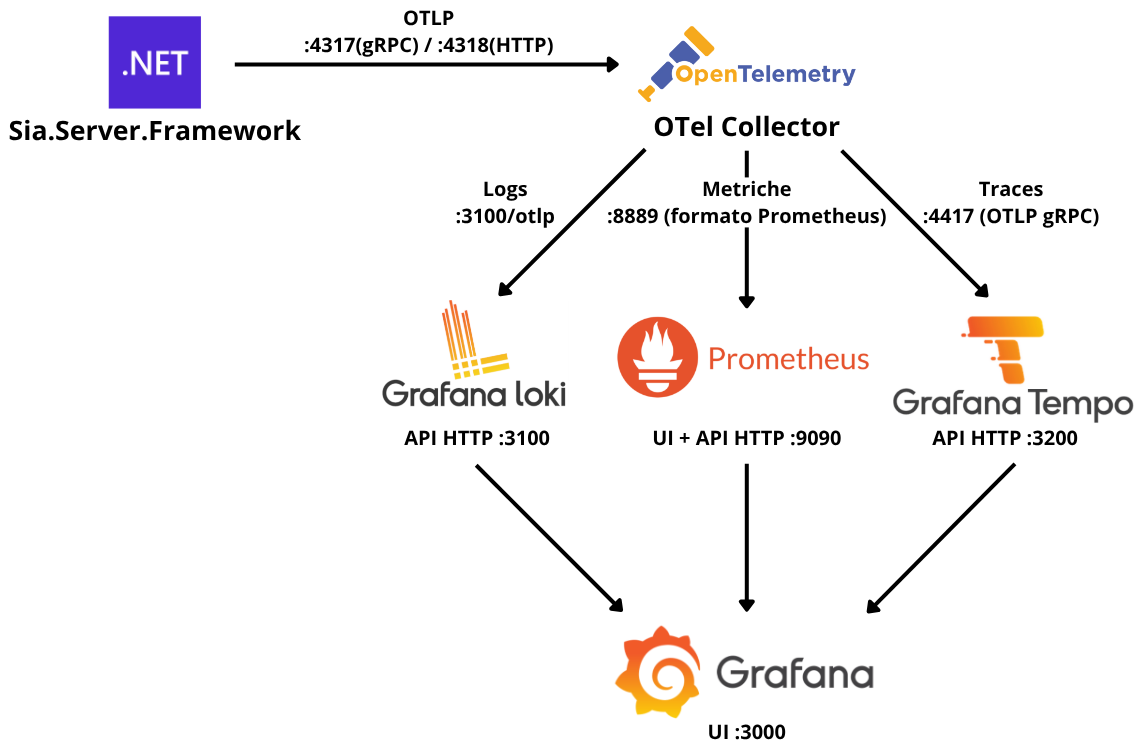
\includegraphics[width=1\linewidth]{../images/architectures/ArchitetturaOtelCollector.png}
    \caption{Architettura OTel Collector}
    \label{fig:arch-otel-collector}
\end{figure}

\subsection{Protocolli e canali di comunicazione}

Ogni segnale telemetrico percorre un canale distinto, scelto in base alle
caratteristiche del dato e ai requisiti di affidabilità del trasporto.\\
L'applicazione .NET invia tutti i segnali all'\gls{otel} Collector attraverso il
protocollo \gls{otlp}, che utilizza \emph{Protobuf} come formato di
serializzazione. \emph{Protobuf} è un formato binario: a parità di informazione
trasportata, occupa una frazione dello spazio di un formato testuale come JSON,
riducendo la banda consumata e il tempo di serializzazione. Per il trasporto,
\gls{otlp} supporta due alternative: \gls{grpcg} sulla porta 4317, che offre
multiplexing delle richieste su una singola connessione persistente ed è il canale
primario del progetto; HTTP sulla porta 4318, mantenuto come canale secondario per
ambienti in cui \gls{grpcg} è bloccato da proxy o firewall.\\
Raccolti dal Collector, i tre segnali vengono instradati verso database separati
con protocolli differenziati. I \emph{log} raggiungono Grafana Loki sulla porta
3100 tramite \gls{otlp} HTTP con serializzazione \emph{Protobuf}. Le \emph{trace}
raggiungono Grafana Tempo sulla porta 4417 tramite \gls{grpcg} con \emph{Protobuf}.
Le \emph{metriche} seguono
invece un percorso diverso: il Collector le espone sulla porta 8889 tramite
\emph{remote write} HTTP con \emph{Protobuf}, e Prometheus le raccoglie con
\emph{scrape} periodico. Questa scelta riflette la natura delle metriche, dati
aggregati e periodici, non eventi discreti, per i quali il modello \emph{pull}
di Prometheus è più efficiente di una connessione persistente.\\
Grafana si connette infine ai tre database tramite HTTP con formato JSON: un
protocollo testuale leggibile, appropriato per le query interattive delle
dashboard dove la latenza di serializzazione è trascurabile rispetto ai tempi
di risposta dell'utente.

\subsection{Scelte architetturali}

\subsubsection{Adozione di OpenTelemetry}

La scelta di \gls{otel}, come richiesto dal requisito RVN-1, permette flessibilità nella scelta
del backend di visualizzazione. 
Le alternative considerate, soluzioni proprietarie come Azure Application Insights o Datadog APM,
avrebbero introdotto un accoppiamento stretto con un singolo fornitore, limitando la
flessibilità nella scelta del backend e rendendo difficoltosa la migrazione futura.

\subsubsection{Architettura opt-in}

L'intero sistema è progettato come \emph{opt-in}: la telemetria è attiva solo se\\
\texttt{OpenTelemetry:Enabled = true} in \emph{appsettings}, rispettando così il requisito RFN-5.
Questo consente di abilitarla esclusivamente negli ambienti che la richiedono, evitando \emph{overhead} in sviluppo locale.

\subsubsection{Centralizzazione della configurazione}

Tutta la configurazione \gls{otel} è centralizzata in \texttt{BaseApplicationBuilder},
componente condiviso da tutti i prodotti \emph{Sia.Web}. I singoli moduli si limitano a
registrare il proprio \texttt{ActivitySource} e \texttt{Meter} nel provider gi\`a
costruito, senza conoscere i dettagli del pipeline.

\subsubsection{Campionamento}

Il campionamento è gestito da un \gls{samplerg} custom, che
combina una logica \emph{ratio-based} per le \emph{root span} con ereditarietà
della decisione per le \emph{child span}.\\
Se lo span ha un parent valido (\texttt{TraceId} e \texttt{SpanId} non nulli),
il \gls{samplerg} eredita la decisione del parent senza ricalcolo. Questo garantisce la
coerenza interna della trace: se la root viene campionata, tutte le child span,
vengono raccolte integralmente.\\
Per le root span, il \gls{samplerg} risolve il ratio da applicare tramite \texttt{ResolveRatio}:
il nome dell'activity (es.\ \texttt{sia.grid.page}) viene confrontato con i prefissi
derivati dai nomi source configurati in appsettings (es.\ \texttt{Sia.Grid}
$\to$ \texttt{sia.grid.}). I prefissi sono ordinati per lunghezza decrescente, così
il match più specifico ha sempre precedenza su quello più generale. Se nessun prefisso
corrisponde, si applica il ratio globale \texttt{SamplingRatio}.

\subsubsection{Arricchimento automatico del contesto utente}
\label{sec:enduser-middleware}

Per soddisfare il requisito RFN-10, il sistema arricchisce automaticamente ogni span con
l'identità dell'utente autenticato senza richiedere modifiche ai singoli moduli applicativi. Il
meccanismo è descritto nel dettaglio nella sezione~\ref{sec:modello-enduser}.

\subsubsection{Correlazione metrica-trace tramite \emph{exemplars}}
\label{sec:exemplars-design}

Per soddisfare il requisito RFN-11, le metriche di tipo \emph{Histogram} espongono
\emph{exemplars}, ovvero campioni che portano con sé il \texttt{TraceId} della richiesta che li ha
generati. Questo abilita la navigazione dal pannello di una metrica aggregata alla trace
specifica che ha prodotto il campione anomalo, risolvendo la domanda ``quale richiesta ha
causato questo picco?''. Il meccanismo è descritto nel dettaglio nella
sezione~\ref{sec:modello-exemplars}.

\subsubsection{Pattern architetturali applicati}
\label{sec:design-patterns-intro}

La soluzione si appoggia a due \emph{design pattern} classici per risolvere problemi ricorrenti:
il pattern \emph{Adapter}, utilizzato per riconciliare i \texttt{Counter} per-modulo con un
contratto comune (\texttt{IControllerDiagnostics}), e il pattern \emph{Factory}, utilizzato per
costruire gli oggetti del pipeline \gls{otel} a partire dalla configurazione \emph{appsettings}.
I dettagli sono illustrati nella sezione~\ref{sec:design-patterns}.

\section{Modello dei segnali e utilizzo degli attributi}
\subsection{Modello dei log}

I log sono prodotti da Serilog con l'interfaccia \texttt{ILogger<T>} e arricchiti
automaticamente con \texttt{TraceId} e \texttt{SpanId} quando emessi nel contesto di una
richiesta tracciata. Questo abilita la navigazione bidirezionale tra log e trace in Grafana.

\subsection{Modello delle trace}

Una \emph{trace} \`e l'insieme completo di un'operazione end-to-end, identificata da un
unico \texttt{trace\_id}. \`E composta da una gerarchia di \emph{span}, ciascuno con un
proprio \texttt{span\_id} e, ad eccezione della root, un \texttt{parent\_span\_id}.\\
Nel sistema, le trace sono prodotte da tre tipologie di sorgenti: instrumentazione
automatica HTTP (richieste in ingresso via AspNetCore, chiamate in uscita via HttpClient);
instrumentazione automatica database (query SQL Server via SqlClient, query PostgreSQL via
Npgsql); instrumentazione manuale dei moduli di Sia.Core tramite le classi
\texttt{Sia[NomeModulo]Diagnostics}.

\subsection{Modello delle metriche}

Sono impiegati quattro tipi di metriche, offerti
dall'\gls{api} \texttt{System.Diagnostics.Metrics} di \emph{.NET}:

\begin{description}
  \item[Counter] Contatore monotono crescente per eventi cumulativi (es.\ login riusciti,
    query eseguite). In Prometheus acquisisce il suffisso \texttt{\_total}.
  \item[Histogram] Distribuzione statistica per latenze e percentili (p50, p95, p99).
    In Prometheus genera tre serie: \texttt{\_bucket}, \texttt{\_sum}, \texttt{\_count}.
  \item[UpDownCounter] Contatore non monotono, che può essere incrementato o decrementato,
    utilizzato per rappresentare grandezze ``in corso'' (es.\ numero di operazioni attualmente
    in esecuzione).
  \item[ObservableGauge] Strumento campionato tramite \emph{callback} periodica, utilizzato per
    valori istantanei non cumulativi (es. numero di connessioni
    attive).
\end{description}
La progettazione delle metriche ha seguito due criteri guida. Il primo è la bassa cardinalità: 
i tag con alta variabilità (es. identificatori numerici di record) sono
applicati solo agli span, mai alle metriche, per evitare un'esplosione del numero di serie
temporali in Prometheus. Il secondo è la pre-aggregazione: le metriche vengono
aggregate lato applicazione prima dell'esportazione, con overhead nettamente inferiore
rispetto alla raccolta di trace complete.

\subsection{Tassonomia degli attributi}

\subsubsection{Resource attributes (comuni a tutti i segnali)}
Attributi presenti in tutte le metriche, trace e log di tutti i moduli.

\begin{table}[h]
\centering
\caption{Resource attributes comuni a trace, metriche e log}
\label{tab:resource-attrs}
\begin{tabular}{|c|c|c|}
\hline
\textbf{Attributo} & \textbf{Chiave appsettings} & \textbf{Scopo} \\
\hline
\texttt{service.name}       & \texttt{ServiceName}  & Identifica l'installazione \\
\hline
\texttt{sia.product\_type}  & \texttt{ProductType}  & Linea di prodotto \\
\hline
\texttt{sia.customer\_name} & \texttt{CustomerName} & Nome del cliente \\
\hline
\end{tabular}
\end{table}

\subsubsection{Attributi del modulo Sia.Base}
Tutti i tag utilizzati nel modulo Sia.Base, modulo che si occupa delle chiamate \gls{crud} al database, sono i medesimi sia per le trace che per le metriche.

\begin{table}[h]
\centering
\caption{Tag del modulo Sia.Base (operazioni \gls{crud})}
\label{tab:tags-base}
\begin{tabular}{|C{3.5cm}|C{4.5cm}|C{4.5cm}|}
\hline
\textbf{Tag} & \textbf{Significato} & \textbf{Valori esempio} \\
\hline
\texttt{sia.operation}
  & Tipo di operazione \gls{crud}
  & \texttt{insert}, \texttt{update}, \texttt{delete},
    \texttt{find\_one}, \texttt{find\_many},
    \texttt{relaz\_check}, \texttt{custom} \\
\hline
\texttt{sia.method}
  & Metodo infrastrutturale
  & \texttt{InsertSiaEntity}, \texttt{UpdateSiaEntity},
    \texttt{FindSiaEntities} \\
\hline
\texttt{sia.caller\_method}
  & Metodo business chiamante
  & \texttt{CreateOrder}, \texttt{SaveInvoice} \\
\hline
\texttt{sia.entity}
  & Tipo C\# dell'entit\`a
  & \texttt{OrderEntity}, \texttt{UserEntity} \\
\hline
\texttt{sia.repository}
  & Classe repository
  & \texttt{OrdersRepository}, \texttt{CatalogRepository} \\
\hline
\texttt{sia.relaz.kind}
  & Tipo di controllo relazione
  & \texttt{relaz}, \texttt{view-relaz} \\
\hline
\texttt{exception.type}
  & Tipo eccezione (solo errori)
  & \texttt{SqlException}, \texttt{TimeoutException} \\
\hline
\end{tabular}
\end{table}

\subsubsection{Attributi del modulo Sia.Auth}
I tag nelle metriche del modulo Sia.Auth sono a bassa cardinalità, di fatto solo la metrica \texttt{sia.auth.login.failure} contiene il tag \texttt{reason} che decrive il motivo dell'errore.
\\
Mentre le trace, contengono i seguenti attributi:
\begin{table}[h]
\centering
\caption{Tag degli span del modulo Sia.Auth}
\label{tab:tags-auth}
\begin{tabular}{|c|c|}
\hline
\textbf{Tag} & \textbf{Valori possibili} \\
\hline
\texttt{auth.method}                & \texttt{credentials} \\
\hline
\texttt{auth.result}                & \makecell{\texttt{success}, \texttt{unauthorized}, \texttt{error},\\
                                      \texttt{bad\_request}, \texttt{two\_factor\_required}} \\
\hline
\texttt{auth.two\_factor\_required} & \texttt{true} (solo se 2FA richiesto) \\
\hline
\texttt{auth.two\_factor\_type}     & \texttt{email}, \texttt{totp} \\
\hline
\end{tabular}
\end{table}

\subsubsection{Attributi del modulo Sia.Grid}
Le metriche, come le trace del modulo Sia.Grid, contengono tutte l'attributo \texttt{componentId}.

\begin{table}[h]
\centering
\caption{Tag degli span del modulo Sia.Grid}
\label{tab:tags-grid}
\begin{tabular}{|c|c|}
\hline
\textbf{Span} & \textbf{Tag} \\
\hline
\texttt{sia.grid.page}            & \texttt{componentId}, \texttt{hasSpName} \\
\hline
\texttt{sia.grid.summary}         & \texttt{componentId} \\
\hline
\texttt{sia.grid.massive\_delete} & \texttt{componentId}, \texttt{spName} \\
\hline
\end{tabular}
\end{table}

\subsection{Tracciamento dell'identità utente}
\label{sec:modello-enduser}

Ogni trace generata da una chiamata autenticata riporta automaticamente l'identità
dell'utente tramite i tag \texttt{enduser.id} ed \texttt{enduser.name}, senza che i
singoli moduli debbano iniettarli manualmente (RFN-10).\\ 
Il meccanismo si articola in due componenti trasparenti al codice applicativo: 
\begin{description}
  \item[un middleware ASP.NET Core] (\texttt{EnrichActivityWithUserMiddleware}), registrato dopo \texttt{UseAuthentication()},
legge gli attributi \texttt{userId} e \texttt{userName} da \texttt{HttpContext.User} e le
pubblica nel \gls{baggageg} \gls{otel}.
 \item[un \texttt{ActivityProcessor} custom] (\texttt{BaggageActivityProcessor}) intercetta l'hook \texttt{OnStart} di ogni nuova
\texttt{Activity} e copia le entry con prefisso \texttt{enduser.} come tag sullo span.
Poiché il \gls{baggageg} viene ereditato dalle child span, tutte le query SQL generate
nell'ambito della stessa richiesta portano gli stessi \texttt{enduser.*} della root.
\end{description}
Gli attributi \texttt{enduser.*} non vengono mai aggiunti come tag delle metriche: 
farlo farebbe crescere il numero di serie temporali di Prometheus
linearmente con il numero di utenti, violando RQN-2. La correlazione \emph{metrica~$\to$~utente}
si ottiene invece tramite gli exemplar: dalla metrica si naviga alla trace, che porta
già \texttt{enduser.*}.

\subsection{Exemplar: collegamento diretto da metrica a trace}
\label{sec:modello-exemplars}
Le metriche aggregate dicono quanto e quando qualcosa è andato storto, ma
non quale richiesta specifica ne è responsabile. Un picco sul percentile $p_{99}$
della latenza, ad esempio, non rivela di per sé la chiamata incriminata. Gli
\emph{exemplar} colmano questo divario: sono campioni concreti allegati ai dati aggregati
di una metrica che trasportano il \texttt{TraceId} della richiesta che li ha prodotti.
In Grafana, si materializzano come piccoli diamanti sovrapposti ai grafici istogramma;
un click su uno di essi apre direttamente la trace corrispondente in Tempo, dalla quale
si può proseguire verso i log correlati. Il risultato è una catena di navigazione
completa (metrica~$\to$~trace~$\to$~utente~$\to$~log).\\
L'utilizzo degli \emph{exemplar} è possibile grazie ad una feature di \emph{Prometheus}
chiamata \emph{exemplar-storage}. Quest'ultima è stata affiancata al filtro \texttt{TraceBased} 
che risolve il problema dei puntatori orfani, ovvero quei puntatori che puntano ad una trace 
scartata dal sampling. Questa fusione garantisce dunque che un exemplar venga prodotto 
soltanto quando la trace a cui punta è effettivamente
disponibile, azzerando l'overhead sulle richieste non campionate.

\section{Design pattern applicati}
\label{sec:design-patterns}

Oltre ai pattern architetturali generali citati nella sezione~\ref{sec:design-patterns-intro},
la soluzione utilizza due \emph{design pattern} della letteratura classica
\footcite{Book:GoF:DesignPatterns} per risolvere problemi ricorrenti dell'instrumentazione.

\subsection{Pattern Adapter per il counter di errore dei controller}
\label{subsec:pattern-adapter-controller-errors}

\textbf{Contesto}\\ 
In un'architettura a moduli come quella di \emph{Sia.Web}, ogni modulo
possiede una propria classe di diagnostica statica con i propri
\texttt{Counter} e \texttt{Histogram}, registrati sul \texttt{Meter}
specifico del modulo. Questo garantisce isolamento e flessibilità, ma
introduce un rischio di divergenza: la logica di registrazione degli errori
nei controller, che richiede l'\emph{unwrap} di
\texttt{SiaLoggerException.OriginalException} e l'applicazione dei \emph{tag}
\texttt{exception.type} e \texttt{sia.operation}, rischierebbe di essere
replicata in modo leggermente diverso in ciascun controller, rendendo le
metriche non omogenee e difficili da confrontare in Grafana.\\
\\\textbf{Problema}\\
Le classi di diagnostica dei moduli sono \texttt{static} e non possono
implementare direttamente un'interfaccia di istanza. È necessario
riconciliare il contratto astratto fornito dal \emph{framework} con la
pluralità di implementazioni concrete, senza duplicare la logica di
\emph{unwrap} nei singoli controller.\\
\\\textbf{Soluzione}\\
Il \emph{framework} espone un'interfaccia
\texttt{IControllerDiagnostics} con un unico membro
\texttt{Counter<long> ControllerErrors} e un metodo condiviso
\texttt{RecordMetricError(\\IControllerDiagnostics, Exception, string)}
che incapsula la logica di \emph{unwrap} e di applicazione dei \emph{tag}.
Per ciascun modulo viene definita una classe annidata
\texttt{private sealed class ControllerDiagnosticsAdapter}: l'\emph{Adapter}
adatta il \emph{counter} statico del modulo al contratto comune. La classe
\texttt{Sia\{Modulo\}Diagnostics} espone, accanto ai \emph{field} statici
esistenti, un singleton
\texttt{public static readonly IControllerDiagnostics AsControllerDiagnostics};
il controller invoca sempre
\texttt{RecordMetricError(Sia\{Modulo\}Diagnostics.AsControllerDiagnostics, ex,\\ nameof(Metodo))}
senza conoscere l'implementazione concreta.\\
Il listato canonico, riferito al modulo \texttt{Sia.Devextreme.Crud}, è
riportato nell'appendice~\ref{app:listing-adapter}
(listati~\ref{lst:adapter-diagnostics-app} e~\ref{lst:recordmetricerror-call-app}).\\
\\\textbf{Vantaggi.}
\begin{itemize}
    \item contratto unico a livello \emph{framework}, \emph{counter}
        distinti per modulo (cardinalità controllata);
    \item logica di \emph{unwrap} e applicazione dei \emph{tag} scritta una
        sola volta;
    \item zero ripetizione nel controller: ogni \texttt{catch} diventa una
        singola riga;
    \item piena retrocompatibilità con i chiamanti diretti dei \emph{field}
        statici esistenti, che rimangono invariati.
\end{itemize}

\subsection{Pattern Factory}

Il pattern \emph{Factory} è applicato in più punti del pipeline \gls{otel} per mantenere in un
unico luogo la traduzione da configurazione \emph{appsettings} a oggetti del runtime
OpenTelemetry.\\
\\\textbf{Costruzione del \emph{sampler}}\\
La creazione di \texttt{SiaParentBasedSampler}
avviene in un metodo \emph{factory} che, letti il valore globale \texttt{SamplingRatio} e i
\emph{ratio} per-\emph{source} da \emph{appsettings}, restituisce l'istanza del \gls{samplerg}
configurata correttamente. L'invocazione avviene una sola volta in
\texttt{BaseApplicationBuilder}; il resto del pipeline consuma un oggetto già pronto.\\
\\\textbf{Registrazione di \texttt{Meter} e \texttt{ActivitySource}}\\
Le classi
\texttt{Sia\{Modulo\}Diagnostics} agiscono come \emph{static factory} centralizzata per gli
strumenti di osservabilità del modulo: istanziano al \emph{type loading} il \texttt{Meter}, gli
\texttt{ActivitySource}, e i \texttt{Counter}/\texttt{Histogram} esposti come membri statici
pubblici. Il codice applicativo non istanzia mai direttamente uno strumento \gls{otel}, ma accede
sempre all'istanza fornita dalla classe \texttt{Diagnostics} del proprio modulo.\\
\pagebreak
\\\textbf{Costruzione del \texttt{ResourceBuilder}}\\
Gli attributi di \emph{resource}
(\texttt{service.name}, \texttt{sia.product\_type}, \texttt{sia.customer\_name}) vengono letti
da \emph{appsettings} e applicati a un unico \texttt{Resource} condiviso da \emph{trace},
metriche e \emph{log}, garantendone la coerenza cross-segnale. Anche questa costruzione avviene
in un metodo \emph{factory} interno a \texttt{BaseApplicationBuilder}.\\
\\\textbf{Vantaggi}
\begin{itemize}
    \item la configurazione da \emph{appsettings} viene tradotta in oggetti \gls{otel} in un solo
        punto, semplificando i test e le variazioni per ambiente;
    \item i moduli vedono solo istanze pronte all'uso, senza conoscere il pipeline;
    \item è possibile sostituire la \emph{factory} con una variante \emph{mock} per i test
        senza toccare il codice di business.
\end{itemize}

\section{Diagrammi delle classi del sistema di telemetria}
\label{sec:class-diagrams}

A complemento delle descrizioni narrative dei paragrafi precedenti, la
struttura complessiva del sistema di telemetria è formalizzata in tre
diagrammi delle classi in stile \gls{uml} semplificato:

\begin{itemize}
    \item il \emph{pipeline} \gls{otel} centralizzato in
        \texttt{BaseApplicationBuilder}, con i tre \emph{provider}
        (\texttt{TracerProvider}, \texttt{MeterProvider},
        \texttt{LoggerProvider}) che condividono lo stesso
        \texttt{ResourceBuilder} ed esportano via
        \texttt{OtlpExporter} (figura~\ref{fig:diag-pipeline});
    \item la struttura generica del pattern
        \texttt{Sia\{Modulo\}Diagnostics} con il\\
        \texttt{ControllerDiagnosticsAdapter} annidato
        (figura~\ref{fig:diag-diagnostics-pattern});
    \item il flusso di arricchimento automatico delle \texttt{Activity}
        con l'identità utente, dal \emph{middleware} ASP.NET Core al
        \texttt{BaggageActivityProcessor} (figura~\ref{fig:diag-enduser}).
\end{itemize}
Per non interrompere il flusso narrativo del capitolo, i tre diagrammi e le
relative descrizioni di dettaglio sono raccolti nell'appendice~\ref{app:diagrammi-classi}.

\section{Implementazione dei test automatici}

\subsection{Contesto}

Prima dell’intervento, la validazione del comportamento applicativo avveniva
principalmente tramite verifiche manuali dell’interfaccia utente. Questo approccio
rendeva complesso modificare i moduli centrali del framework con sufficiente
sicurezza, poiché ogni cambiamento introduceva il rischio di regressioni difficili
da individuare in modo sistematico.\\
L’assenza di una suite automatizzata comportava inoltre:

\begin{itemize}
    \item la mancanza di una rete di sicurezza durante attività di \emph{refactoring};
    \item tempi elevati per la validazione delle modifiche;
    \item difficoltà nell’individuazione precoce di difetti;
    \item assenza di una \emph{baseline} condivisa sul comportamento atteso del sistema.
\end{itemize}
L’obiettivo dello stage è stato quindi introdurre una metodologia di testing
riproducibile e integrabile nei processi di sviluppo, capace di verificare sia
la correttezza della logica applicativa sia il comportamento dell’interfaccia
utente in scenari realistici.

\subsection{Strategia di testing adottata}

La strategia implementata è stata suddivisa in più livelli, ciascuno dedicato
alla validazione di aspetti differenti del sistema.
La strategia adottata distingue quattro tipologie di test con responsabilità
complementari: Unit test frontend, test \emph{end-to-end} frontend, unit test backend
e integration test backend.
L’introduzione di più livelli di test ha permesso di ottenere una copertura più
ampia del sistema, combinando verifiche veloci e isolate con controlli completi
sul comportamento integrato dell’applicazione.

\subsubsection{Unit test backend}

Gli \emph{unit test} backend hanno l’obiettivo di verificare in isolamento la
logica applicativa implementata lato server, senza coinvolgere componenti esterni
come database reali, servizi remoti o infrastrutture di rete.\\
Questo tipo di test consente di validare rapidamente il comportamento delle
singole unità software, riducendo il rischio di regressioni durante le modifiche
al codice e facilitando le attività di manutenzione e \emph{refactoring}.\\
Nel progetto sviluppato durante lo stage, tali test sono stati utilizzati per
validare il comportamento dei servizi applicativi del framework e delle API
utilizzate dal frontend. In particolare, sono state verificate la corretta
gestione delle richieste, la propagazione delle eccezioni, il comportamento
dei repository e la logica associata ai moduli instrumentati con OpenTelemetry.\\
L’utilizzo di dipendenze simulate (\emph{mock}) ha permesso di eseguire i test
in modo deterministico e veloce, senza richiedere l’avvio dell’intera
infrastruttura applicativa.

\subsubsection{Integration test backend}

I test di integrazione backend verificano il corretto funzionamento congiunto
dei diversi componenti dell’applicazione: accesso al database, persistenza dei dati,
serializzazione, servizi applicativi e infrastruttura del framework.
A differenza degli \emph{unit test}, questi test non isolano le dipendenze tramite
\emph{mock}, ma eseguono operazioni reali su un ambiente controllato, così da
riprodurre scenari più vicini al comportamento effettivo del sistema in produzione.\\
Nel progetto sono state adottate tre tipologie principali di test di integrazione.
La prima riguarda i test \gls{crud},
chiamati \textbf{lifecycle test}, come suggerito dal nome, verificano l'intero ciclo di vita 
di un entità sul database, controllando che tutte e quattro le operazioni vadano a termine correttamente.\\
La seconda categoria, \textbf{smoke test}, ha lo scopo di esercitare ogni singola configurazione 
per componente presente in produzione,
intercettando \emph{stored procedure} malformate, \emph{connection name} non
risolvibili o configurazioni errate di colonne. Iterando su tutti i componenti 
presenti nel database e per ciascuno 
effettua una chiamata reale all'\emph{endpoint} di lettura
(es. \texttt{POST /api/grid-core/page} o \texttt{GET /api/CrudData/page}),
asserendo che la risposta sia \texttt{200 OK} con \emph{payload} JSON valido. \\
Infine, sono presenti \textbf{test summary} specifici per i componenti griglia, durante i quali
vengono testati gli \emph{endpoint} responsabili del calcolo aggregato (\texttt{sum}, 
\texttt{avg}, \texttt{count}, \texttt{min}, \texttt{max}), verificando che le 
colonne configurate (tramite \emph{perspective} JSON) con funzionalità di aggregazione, funzionino correttamente.\\
L’utilizzo di dati reali provenienti dal database consente di validare non solo
la correttezza del codice applicativo, ma anche l’affidabilità e la consistenza
dei dati presenti nel sistema. Questo approccio permette di individuare problemi
che difficilmente emergerebbero tramite semplici \emph{mock}, come incongruenze
nei dati, errori di mapping, vincoli non rispettati o differenze tra schema
atteso e stato effettivo del database.

\subsubsection{Unit test frontend}

Gli \emph{unit test} sono scritti con \textbf{Vitest} e hanno l’obiettivo di verificare
in isolamento le singole unità logiche dell’applicazione frontend, senza coinvolgere
componenti esterni come il browser, il \emph{backend} o il \emph{rendering} reale
dell’interfaccia grafica.  
Questo tipo di test permette di validare il comportamento di funzioni, servizi e
componenti applicativi in modo rapido e deterministico, riducendo il rischio di
regressioni durante l’evoluzione del software.\\
In generale, gli \emph{unit test} verificano aspetti quali:
\begin{itemize}
    \item la correttezza della logica applicativa;
    \item la gestione dello stato interno dei componenti;
    \item la trasformazione e validazione dei dati;
    \item la gestione degli errori e dei casi limite;
    \item il corretto comportamento di metodi puri e funzioni di utilità.
\end{itemize}
Nel progetto sviluppato durante lo stage, i test hanno riguardato principalmente
la logica frontend implementata in TypeScript, includendo servizi applicativi,
componenti Angular e direttive personalizzate. In particolare, sono stati verificati
la gestione dello stato
dei componenti, i meccanismi di raccolta e filtraggio dei dati, oltre al comportamento
di funzionalità interattive come selezione, ordinamento e aggiornamento dinamico
dell’interfaccia.\\
Questi test non richiedono né un browser reale né servizi esterni attivi, risultando
quindi molto veloci nell’esecuzione e facilmente integrabili nei processi automatici
di validazione del software.

\subsubsection{Test end-to-end con Playwright}

I test \emph{end-to-end} (\emph{E2E}) sono stati sviluppati tramite
\textbf{Playwright} e hanno lo scopo di verificare il comportamento
complessivo dell’applicazione simulando l’interazione di un utente reale
con l’interfaccia web.\\
A differenza degli unit test, i test E2E eseguono l’applicazione in un browser
reale e validano l’integrazione tra frontend, backend e servizi coinvolti.
Questo approccio permette di intercettare problemi che emergono solo durante
l’esecuzione completa del sistema, come errori di rendering, problemi di
sincronizzazione, regressioni dell’interfaccia o malfunzionamenti nei flussi
utente.\\
Come esposto precedentemente i test E2E sono utilizzati per verificare
l'esperienza utente, in questa categoria ricadono requisiti come:
la corretta navigazione tra le pagine, il comportamento delle principali 
funzionalità applicative, la corretta visualizzazione degli elementi grafici,
la persistenza e l’aggiornamento dei dati nell’interfaccia grafica.
Nel progetto, tali test sono stati utilizzati per validare il comportamento
reale dei componenti più complessi del framework, come griglie dati,
form dinamiche, operazioni \gls{crud} e flussi di autenticazione.
Sono stati inoltre utilizzati per verificare la corretta propagazione delle
modifiche introdotte dagli agenti AI, riducendo il rischio di regressioni
funzionali nei moduli condivisi.
Il costo da pagare è la velocità di esecuzione:
ogni test richiede secondi, non millisecondi e la dipendenza dallo stato del
sistema. Per questo i test E2E si concentrano sui flussi utente strategici,
lasciando la copertura della logica di dettaglio agli \emph{unit test}.

\subsection{Vantaggi ottenuti}

L'impatto più immediato dell'introduzione dei test è stata la scoperta di difetti
latenti che non sarebbero emersi prima di un incidente in produzione.
Per gli sviluppi futuri invece, l’automazione dei test ha reso possibile l’integrazione 
delle verifiche all’interno del flusso di sviluppo quotidiano, riducendo il numero di
regressioni e migliorando la qualità complessiva del processo di sviluppo.
L’esecuzione automatica delle suite ha ridotto significativamente il tempo
necessario alla validazione delle modifiche e ha aumentato la confidenza nei
refactoring dei moduli centrali del framework.
Inoltre, la disponibilità di test automatici si è rivelata particolarmente utile nel
contesto dello sviluppo AI-assistito: gli agenti di codifica potevano infatti
produrre modifiche su più moduli, mentre le suite automatiche fornivano una
validazione immediata del comportamento atteso.
